\documentclass[12pt]{article}  % default square logo

\usepackage[margin=2.8cm]{geometry}
\usepackage{setspace}
\usepackage{mathptmx} % Times font
\usepackage[utf8]{inputenc}

% handles ~ in url
\usepackage{hyperref}

% center captions
\usepackage[justification=centering]{caption}

% code listing
\usepackage{listings}
\usepackage{xcolor}

% packages for drawing
\usepackage{tikz}
\usetikzlibrary{graphs}     % create graphs

% for warning box
\usepackage{pifont,mdframed}
\usepackage{framed}

% algorithms
\usepackage[]{algorithm}
\usepackage[]{algpseudocode}

% tables
\usepackage{tabularx}         % full-width

%%%%%%%%%%%%%%%%%%%%%%%%%%%%%%%%%%%%%%%%%%%%%%%%%%%%%%%%%%%%%%%%%%%%%%%%%%%%%%%%%%%%%%%%%

\onehalfspacing

%% styles for filter graph
\tikzstyle{filter} = [rectangle, draw, font=\small, text centered, rounded corners, minimum height=2em, node distance=3cm, minimum width=4em]

%% set code styles

\definecolor{dkgreen}{rgb}{0,0.6,0}
\definecolor{gray}{rgb}{0.5,0.5,0.5}
\definecolor{mauve}{rgb}{0.58,0,0.82}

\lstset{
  frame=tb,
  language=scala,
  aboveskip=3mm,
  belowskip=3mm,
  showstringspaces=false,
  columns=flexible,
  basicstyle={\small\ttfamily},
  numbers=none,
  numberstyle=\tiny\color{gray},
  keywordstyle=\color{blue},
  commentstyle=\color{dkgreen},
  stringstyle=\color{mauve},
  breaklines=true,
  breakatwhitespace=true,
  tabsize=3,
}

%% warning box

\newenvironment{warning}
               {\par\begin{mdframed}[linewidth=1pt,linecolor=red!20,backgroundcolor=yellow!40]%
                 \begin{list}{}{\leftmargin=1cm
                     \labelwidth=\leftmargin}\item[\Large\ding{43}]}
               {\end{list}\end{mdframed}\par}

\newenvironment{info}
               {\par\begin{mdframed}[linewidth=1pt,backgroundcolor=blue!20!white]%
                 \begin{list}{}{\leftmargin=1cm
                     \labelwidth=\leftmargin}\item[\Large\ding{46}]}
               {\end{list}\end{mdframed}\par}

%%%%%%%%%%%%%%%%%%%%%%%%%%%%%%%%%%%%%%%%%%%%%%%%%%%%%%%%%%%%%%%%%%%%%%%%%%%%%%%%%%%%%%%%%
\begin{document}

\begin{titlepage}

  \begin{center}

    %% \vspace{20cm}
    \vspace*{3\baselineskip}
    % Title
    {\Large \bfseries Programming Guide for TradingSimulation \\[0.4cm] }

    % Author and supervisor
    \noindent
    TradingSimulation Developer Team \\[4cm]

    \begin{framed}
    Project of Big Data Course \\
    Professor: Christoph Koch \\
    \end{framed}

    \noindent
    Lausanne, Academic Year 2014 - 2015 \\[1cm]

    % Upper part of the page. The '~' is needed because \\
    % only works if a paragraph has started.
    
\includegraphics[width=0.8\textwidth]{img/epfl}~\\[1cm]

    \vfill

    % Bottom of the page
    {\large \today}

  \end{center}

\end{titlepage}

\subsection*{Preface}

The targeted audience of this documentation is developers who want to use the TradingSimulation framework to experiment with algorithmic trading or contribute to the TradingSimulation project. The readers should have some background in algorithmic trading or have access to expertises of the field. The reader should also be familiar with programming in Scala.


%% \pagenumbering{Roman}
\tableofcontents

%% \pagenumbering{arabic}

%!TEX root = ../guide.tex

\section{Introduction}
\label{sec:1}

This section introduces the functionalities, use cases and architecture of the TradingSimuation framework.

\subsection{What's TradingSimulation}

TradingSimulation is an open source\footnote{\url{https://github.com/merlinND/TradingSimulation}} algorithmic trading framework based on Scala\footnote{\url{http://scala-lang.org}}. The framework provides a lot of standardized components, which can be easily composed by the programmers with a few lines of Scala code to do various experiments related to algorithmic trading.

Following are a list of use cases of TradingSimulation:

\begin{itemize}
\item Simulation of multiple traders in a virtual market
\item Evaluation of a trading algorithm against live Forex data
\item Evaluation of a trading algorithm against live Bitcoin data
\item Evaluation of a trading algorithm based on historical market data
\end{itemize}

\subsection{The Architecture of TradingSimulation}

The design of TradingSimulation is based on the \emph{Pipes and Filters}\footnote{\url{http://www.cs.olemiss.edu/~hcc/csci581oo/notes/pipes.html}} architectural pattern, which results in a very high level of modularity, extensibility and reusability of the framework.

In the terminology of \emph{Pipes and Filters}, the standard components provided by the TradingSimulation framework are called \emph{filters}. The programmers can select appropriate filters and connect them properly according to the specific experiment purpose. Each configuration of filters is called a \emph{filter graph}.

Figure~\ref{fig-filter-graph} is an example filter graph of TradingSimulation. In the filter graph, there are six inter-connected filters.


\begin{figure}
  \centering
  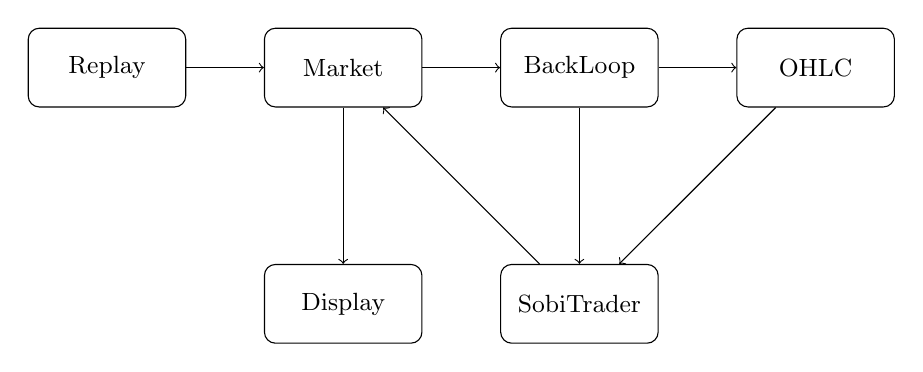
\begin{tikzpicture}[every node/.style={rectangle, draw, font=\small, text centered, rounded corners, node distance=3cm, minimum height=1cm, minimum width=2cm}]
    \node (Replay) {Replay};
    \node [right of=Replay] (Market) {Market};
    \node [right of=Market] (BackLoop) {BackLoop};
    \node [right of=BackLoop] (OHLC) {OHLC};
    \node [below of=BackLoop] (SobiTrader) {SobiTrader};
    \node [below of=Market] (Display) {Display};

    \graph [grow right=3cm] {
      (Replay) -> (Market) -> { (BackLoop) -> { (OHLC) -> (SobiTrader), (SobiTrader) }, (Display) };
      { (SobiTrader) } -> (Market);
    };
  \end{tikzpicture}
  \centering
  \caption{A Filter Graph in TradingSimulation}
  \label{fig-filter-graph}
\end{figure}

The functions of the filters in Figure~\ref{fig-filter-graph} are explained as follows:

\begin{itemize}
\item{Replay}: Read historical market order data from file system and send them one by one at a constant rate to connected filters. Replay is also called \emph{source filter}, as it doesn't have any input from other filters.
\item{Market}: Receive market orders, create transactions from matching bid and ask orders according to the configured market rules, and send transaction data to connected filters.
\item {BackLoop}: It's a utility filter, which sends everything it receives from input to output.
\item {OHLC}: It receives transaction data and send the prices of Opening, Highest, Lowest and Closing once a time in a configured interval.
\item {Display}: As its name suggests, this filter shows the data it receives in the terminal. It's also called \emph{sink filter}, as it doesn't send any data to other filters.
\item {SobiTrader}: This filter is a trader who employs the \emph{Static Order Book Imbalance}(SOBI) trading strategy. It receives market data such as orders, transactions and OHLC, and sends bid or ask orders to the \emph{Market}.
\end{itemize}

\subsection{A Simple Example}

Following code snippet is intended to give you some feel on how to create and run a filter graph in TradingSimulation.

\lstinputlisting[language=Scala]{code/simple.scala}

As you see in the code, it first creates a component builder, then uses the builder to create various  components, connects the components, and finally starts the graph.

All usages of TradingSimulation have the same form of code as shown in the code snippet, the difference lies in what components are created, what parameters are configured for components, and how components are connected.

For more and complete examples, please check our code repository here\footnote{\url{https://github.com/merlinND/TradingSimulation/tree/master/ts/src/main/scala/ch/epfl/ts/example}}.

\section{Components}
\label{sec:2}

This section introduces each component in detail, including  what data they expect, what data they output, what parameters can be set. After reading this section, you should able to select appropriate components for a specific algorithmic trading purpose, parameterize and connect them correctly.

\subsection{Define a Component}

In TradingSimulation, each component is an Akka\footnote{\url{http://akka.io}} actor. This can be seen from following code snippet, in which the abstract class \emph{Component} indirectly extends the trait \emph{Actor} in Akka. All concrete components extend \emph{Component}.

\begin{lstlisting}[language=Scala]
  trait Receiver extends Actor {
    def receive: PartialFunction[Any, Unit]

    def send[T: ClassTag](t: T): Unit
    def send[T: ClassTag](t: List[T]): Unit
  }

  abstract class Component extends Receiver {
    def start: Unit = {}

    def stop: Unit = {}

    def receiver: PartialFunction[Any, Unit]
  }
\end{lstlisting}

The framework defines three standard methods for every concrete component class:

\begin{itemize}
\item{start}: concrete components can override this method to do custom initialization.
\item{stop}: concrete components can override this method to release resources.
\item{receiver}: concrete components override this method to receive and handle messages.
\end{itemize}

The data transer between different components is in the form of Akka messages. Concrete component classes have to override the method \emph{receiver} in order to handle the messages they are interested in.

To send a message, a concrete component class can call one of the two \emph{send} methods defined in \emph{Receiver}. The two \emph{send} methods have default implementation in \emph{Component}, a concrete component class should not override them.

Following code snippet illustrates a very simple component which just prints and forwards every message it receives.

\begin{lstlisting}[language=Scala]
  class BackLoop extends Component {
    override def receiver = {
      case m =>
        println(m)
        send(m)
    }
  }
\end{lstlisting}

\subsubsection{Create Instances of Components}

To create an instance of a component, we have to first create a \emph{component builder} as follows:

\begin{lstlisting}[language=Scala]
val builder = new ComponentBuilder("test")
\end{lstlisting}

Now suppose we have a Component \emph{Arbitrageur} defined as follows:

\begin{lstlisting}[language=Scala]
  class Arbitrageur(id: Long, delta: Double, volume: Double) extends Component
  {
    //...
  }
\end{lstlisting}

Then we can create an instance of \emph{Arbitrageur} with following code snippet:

\begin{lstlisting}[language=Scala]
  val props = Props(classOf[Arbitrageur], 111L, 1, 50)
  val arbitrageur = builder.createRef(props, "arbitrageur")
\end{lstlisting}

As you can see in the code snippet above, first we create an instance of \emph{Props}\footnote{\url{http://doc.akka.io/api/akka/2.3.1/index.html\#akka.actor.Props}}. The first argument to \emph{Props} is the class we want to instantiate, and the remaining arguments are exactly the parameters that the constructor of the class \emph{Arbitrageur} expects.

\emph{builder.createRef} then takes \emph{props} and a name for the component to create an instance of the component. Note that the return value of \emph{builder.createRef} is a pointer to an instance of \emph{ComponentRef} instead of \emph{Arbitrageur}.

We have learned how to created instances of components, next let's see how to connect them.

\begin{info}
Internally, \emph{builder.createRef} will call \emph{actorOf} on an instance of \emph{ActorSystem} to create an instance of the component. The whole process seems a little awkward, but that's how Akka works. If you ever have a chance to checkout Akka(\href{http://akka.io}{akka.io}), you'll find it's worth the pain.
\end{info}

\subsubsection{Connect Components}

To connect an upstream component A to a downstream component B, we need to specify what types of messages B expects to receive from A. During the running A would only send messages of the specified types to B. For example, in the following code snippet, \emph{sobiTrader} will only send \emph{LimitBidOrder} messages to \emph{market}, and only send \emph{LimitAskOrder} messages to \emph{display}.

\begin{lstlisting}[language=Scala]
  sobiTrader -> (market, classOf[LimitBidOrder])
  sobiTrader -> (display, classOf[LimitAskOrder])
\end{lstlisting}

A downstream component can register as many message types as the upstream component can provide. For example, in the following code snippet \emph{sobiTrader} would send both \emph{LimitBidOrder} and \emph{LimitAskOrder} messages to \emph{market}.

\begin{lstlisting}[language=Scala]
  sobiTrader -> (market, classOf[LimitBidOrder], classOf[LimitAskOrder])
\end{lstlisting}

If a downstream component registers a message type that the upstream component can't provide, the registration has no effect. In practice, it's important to check carefully what messages a component can receive and provide.

Following list are all the types messages that are exchanged between components:

\begin{itemize}
\item Transaction
\item LimitBidOrder
\item LimitAskOrder
\item MarketBidOrder
\item MarketAskOrder
\item DelOrder
\item Quote
\item OHLC
\item MA
\end{itemize}

\subsection{Simulators}

Details of various simulators

\begin{itemize}
\item MarketSimulator
\item MarketFxSimulator
\end{itemize}

\subsection{Indicators}

Details various indicators

\begin{itemize}
\item MA
\item EMA
\item SMA
\item OHLC
\end{itemize}

\subsection{Traders}

Details of various traders

\begin{itemize}
\item Arbitrageur
\item DoubleCrossOverTrader
\item DoubleEnvelopeTrader
\item SimpleFXTrader
\item SimplerTrader
\item SobiTrader
\item TransactionVmapTrader
\end{itemize}

\subsection{Fetchers}

Details of various fecthers

\begin{itemize}
\item BitfinexFetcher
\item BitStampFetcher
\item BtceFetcher
\item CSVFetcher
\item TrueFXFetcher
\end{itemize}

\subsection{Utilities}

Other components

\begin{itemize}
\item Printer
\item Backloop
\item Replay
\item BatcherComponent
\end{itemize}

\section{Catalog of Components}

This section introduces each component that TradingSimulation provides in detail, including what data they expect, what data they output, what parameters can be set.

After reading this section, you should able to select appropriate components for a specific algorithmic trading purpose, parameterize and connect them correctly.

\subsection{Market Simulators}

Market simulators are core components of TradingSimulation, which simulate virtual markets. Market simulators accept ask and bid orders and generate transactions based on \emph{market rules}. In the implementation, market rules are extracted into separate modules to make it possible to define custom market rules and use it in the framework.

Currently TradingSimulation provides two market simulators:

\begin{itemize}
\item OrderBookMarketSimulator
\item MarketFxSimulator
\end{itemize}

\emph{OrderBookMarketSimulator} is usually used to simulate the trading of bitcoins, while \emph{MarketFxSimulator} is used for Forex markets. The Forex market has high liquidity, so it doesn't need order books.

\subsubsection{OrderBookMarketSimulator}

\begin{tabularx}{\textwidth}{|c|X|}
  \hline
  \multicolumn{2}{|c|}{\sc{Parameters}} \\
  \hline
  id: Long  & The market id. It takes one of following values: \emph{MarketNames.BTCE\_ID}, \emph{MarketNames.BITSTAMP\_ID},  \emph{MarketNames.BITFINEX\_ID}. \\
  \hline
  rules: MarketRules & The market rules. The value should be an instance of \emph{MarketRules}, which internally uses order book. \\
  \hline
\end{tabularx}\\[0.4cm]

\noindent
\begin{tabularx}{\textwidth}{|c|X|}
  \hline
  \multicolumn{2}{|c|}{\sc{Message Input}} \\
  \hline
  LimitBidOrder  & the limit bid order from traders or brokers \\
  \hline
  LimitAskOrder  & the limit ask order from traders or brokers \\
  \hline
  MarketBidOrder  & the market bid order from traders or brokers \\
  \hline
  MarketAskOrder  & the market ask order from traders or brokers \\
  \hline
  DelOrder  & the delete order command from traders or brokers \\
  \hline
  PrintBooks  & prints the order book \\
  \hline
\end{tabularx}\\[0.4cm]

\noindent
\begin{tabularx}{\textwidth}{|c|X|}
  \hline
  \multicolumn{2}{|c|}{\sc{Message Output}} \\
  \hline
  Transaction  & the transactions to inform traders or brokers \\
  \hline
  DelOrder  & the delete order to inform traders or brokers \\
  \hline
\end{tabularx}\\[0.4cm]

To create an instance of \emph{OrderBookMarketSimulator}, following code snippet can be used:

\begin{lstlisting}[language=Scala]
val rules = new MarketRules()
val btceMarket = builder.createRef(Props(classOf[OrderBookMarketSimulator], MarketNames.BTCE_ID, rules), MarketNames.BTCE_NAME)
\end{lstlisting}


\subsubsection{MarketFxSimulator}

\begin{tabularx}{\textwidth}{|c|X|}
  \hline
  \multicolumn{2}{|c|}{\sc{Parameters}} \\
  \hline
  id: Long  & The market id. It usually takes the value \emph{MarketNames.FOREX\_ID}. \\
  \hline
  rules: MarketRules & The market rules. The value should be an instance of \emph{ForexMarketRules}. \\
  \hline
\end{tabularx}\\[0.4cm]

\noindent
\begin{tabularx}{\textwidth}{|c|X|}
  \hline
  \multicolumn{2}{|c|}{\sc{Message Input}} \\
  \hline
  LimitBidOrder  & the limit bid order from traders or brokers \\
  \hline
  LimitAskOrder  & the limit ask order from traders or brokers \\
  \hline
  MarketBidOrder  & the market bid order from traders or brokers \\
  \hline
  MarketAskOrder  & the market ask order from traders or brokers \\
  \hline
  Quote  & the quote from live fetcher or playback  \\
  \hline
\end{tabularx}\\[0.4cm]

\noindent
\begin{tabularx}{\textwidth}{|c|X|}
  \hline
  \multicolumn{2}{|c|}{\sc{Message Output}} \\
  \hline
  Transaction  & the transactions to inform traders or brokers \\
  \hline
  Quote  & the quote to inform traders or brokers \\
  \hline
\end{tabularx}\\[0.4cm]

To create an instance of \emph{MarketFxSimulator}, following code snippet can be used:

\begin{lstlisting}[language=Scala]
val rules = new ForexMarketRules()
val forexMarket = builder.createRef(Props(classOf[MarketFXSimulator], MarketNames.FOREX_ID, rules), MarketNames.FOREX_NAME)
\end{lstlisting}

\subsection{Indicators}

Indicators measure the activities of the market. Traders depend on indicators to make sell or buy decisions. Currently TradingSimulation provides following indicators:\\

\noindent
\begin{tabularx}{\textwidth}{|c|X|}
  \hline
  Class & Description  \\
  \hline
  SmaIndicator & Simple Moving Average \\
  \hline
  EmaIndicator & Exponential Moving Average  \\
  \hline
  OhlcIndicator & OHLC(Open-high-low-close)  \\
  \hline
\end{tabularx}\\[0.3cm]

Normally you don't have the need to create indicators, as the traders automatically create indicators that they depend on.

\subsection{Traders}

Traders buy or sell in the virtual market. Different types of traders use different trading strategies. The same strategy may take different parameters thus perform differently. Currently TradingSimulation provides following indicators:\\

\noindent
\begin{tabularx}{\textwidth}{|c|X|}
  \hline
  Class & Description  \\
  \hline
  Arbitrageur & the \emph{arbitrageur} strategy \\
  \hline
  DoubleCrossOverTrader & the \emph{double cross over} strategy  \\
  \hline
  DoubleEnvelopeTrader & the \emph{double envelope} strategy  \\
  \hline
  SobiTrader & the \emph{static order book imbalance} strategy  \\
  \hline
  TransactionVwapTrader & the \emph{volume weighted average price} strategy  \\
  \hline
  SimpleTrader & a simple trader \\
  \hline
  SimpleFXtrader & a simple Forex trader \\
  \hline
\end{tabularx}

\subsection{Fetchers}

Fetchers in TradingSimulation play the role of feeding market data from external sources(internet or file system) into market simulator. Currently TradingSimulation provides following fetchers:\\

\noindent
\begin{tabularx}{\textwidth}{|l|X|}
  \hline
  Class & Description  \\
  \hline
  BtceOrderPullFetcher & the fetcher for BTC-e orders \\
  \hline
  BtceTransactionPullFetcher  & the fetcher for BTC-e transactions  \\
  \hline
  BitfinexOrderPullFetcher & the fetcher for Bitfinex orders  \\
  \hline
  BitfinexTransactionPullFetcher & the fetcher for Bitfinex transactions  \\
  \hline
  BitstampOrderPullFetcher & the fetcher for Bitstamp orders  \\
  \hline
  BitstampTransactionPullFetcher & the fetcher for Bitstamp transactions \\
  \hline
  TrueFxFetcher & the fetcher for  live Forex quotes  \\
  \hline
  HistDataCSVFetcher & reads data from csv source and converts it to Quotes \\
  \hline
\end{tabularx}\\[0.3cm]

Note that all the fetchers in the table above are not components themselves, except \emph{HistDataCSVFetcher}. Non-component fetchers are used together with \emph{PullFetchComponent} as following snippet shows:

\begin{lstlisting}[language=Scala]
  val fetcherFx: TrueFxFetcher = new TrueFxFetcher
  val fetcher = builder.createRef(Props(classOf[PullFetchComponent[Quote]], fetcherFx, implicitly[ClassTag[Quote]]), "TrueFxFetcher")
\end{lstlisting}

\subsubsection{HistDataCSVFetcher}

This uses historical quote data from the free financial data provider histdata.com\footnote{More specifically http://www.histdata.com/download-free-forex-data/?/ninjatrader/tick-\{ask, bid\}-quotes}. The data we used can be comfortably fetched by using our \texttt{get-data.sh} script. For example,  following command can be used to get a set of CSV files to  \lstinline|./data/EURCHF|.

\begin{verbatim}
   scripts/get-data.sh www.histdata.com EURCHF
\end{verbatim}

HistDataCSVFetcher can take this data and send quotes ``replaying'' the past. To build a fetcher replaying EUR/CHF data from April 2013 through May 2013 with a speed factor of 60x (i.e. 1 hour is replayed in 1 minute) the following can be done:

\begin{lstlisting}[language=Scala]
    // variables for the fetcher
    val dateFormat = new java.text.SimpleDateFormat("yyyyMM")
    val startDate = dateFormat.parse("201304");
    val endDate   = dateFormat.parse("201305");
    val workingDir = "./data";
    val currencyPair = "EURCHF";
    val speed = 60;

    // build fetcher
    val fetcher = builder.createRef(Props(classOf[HistDataCSVFetcher], workingDir, currencyPair, startDate, endDate, speed),"HistFetcher")
\end{lstlisting}

The fetcher reads the data from the local file system directly. It looks for directories named after the currency pair that's being fetched in the directory you supply to it. In the example above the source directory is \lstinline|data| and should be structured something like the following:

\begin{lstlisting}
data/
*- EURCHF/
|   ...
|   *- DAT_NT_EURCHF_T_ASK_201304.csv
|   *- DAT_NT_EURCHF_T_ASK_201305.csv
|   ...
*- USDCHF/
    *- DAT_NT_USDCHF_T_ASK_200301.csv
    *- DAT_NT_USDCHF_T_ASK_200302.csv
    ...
    *- DAT_NT_USDCHF_T_BID_200306.csv
    *- DAT_NT_USDCHF_T_BID_200307.csv
    ...
*- ...
\end{lstlisting}

\subsection{Persistors}

Persistors load data from and save data to SQLite database. Currently TradingSimulation provides following persistors:

\noindent
\begin{tabularx}{\textwidth}{|l|X|}
  \hline
  Class & Description  \\
  \hline
  OrderPersistor & loads or saves orders from or to database \\
  \hline
  TransactionPersistor  & loads or saves transactions from or to database  \\
  \hline
  QuotePersistor & loads or saves quotes from or to database  \\
  \hline
\end{tabularx}\\[0.3cm]

Note that none of the persistors above are components themselves. They have to be used together with other classes depending one the scenario.

\subsubsection{Storing Data to Database}

To store data to database, the persistors can be used together with the class \emph{Persistor}. The definition of \emph{Persistor} is as follows:

\begin{lstlisting}[language=Scala]
  class Persistor[T: ClassTag](p: Persistance[T]) extends Component {
    // ...
  }
\end{lstlisting}

We can see that the class \emph{Persistor} takes an object of \emph{Persistance} as parameter. Following code illustrates how to use them together:

\begin{lstlisting}[language=Scala]
  // Initialize the Interface to DB
  val btceXactPersit = new TransactionPersistor("btce-transaction-db-batch")
  btceXactPersit.init()

  val btcePersistor = builder.createRef(Props(classOf[Persistor[Transaction]], btceXactPersit, implicitly[ClassTag[Transaction]]), "btcePersistor")
\end{lstlisting}

\subsubsection{Loading Data from Database}

To load data from database, the persistors can be used together with the class \emph{Replay}. The definition of \emph{Replay} is as follows:

\begin{lstlisting}[language=Scala]
  class Replay[T: ClassTag](p: Persistance[T], conf: ReplayConfig) extends Component {
    // ...
  }
\end{lstlisting}

We can see that the class \emph{Replay} takes an object of \emph{Persistance} as parameter. Following code illustrates how to use persistors together with \emph{Replay}:

\begin{lstlisting}[language=Scala]
  // Initialize the Interface to DB
  val btceXactPersit = new TransactionPersistor("btce-transaction-db")
  btceXactPersit.init()

  // Configuration object for Replay
  val replayConf = new ReplayConfig(1418737788400L, 0.01)

  val replayer = builder.createRef(Props(classOf[Replay[Transaction]], btceXactPersit, replayConf, implicitly[ClassTag[Transaction]]), "replayer")
\end{lstlisting}

\subsection{Miscellaneous}

TradingSimulation also provide some utility components as shown in the table below.\\

\noindent
\begin{tabularx}{\textwidth}{|l|X|}
  \hline
  Class & Description  \\
  \hline
  Printer & prints anything it receives in the console \\
  \hline
  Backloop  & saves transaction to database and forward, similar to the UNIX command \emph{tee}  \\
  \hline
  Evaluator & evaluates the performance of traders\\
  \hline
\end{tabularx}\\[0.3cm]

\section{Usage Scenarios}
\label{sec:3}

This section introduces how to use the framework for common usage scenarios. The examples are at the high level, no code is provided. If you want to refer to concrete examples in code, please refer to the package \emph{ch.epfl.ts.example} or check it out on \href{https://github.com/merlinND/TradingSimulation/tree/master/ts/src/main/scala/ch/epfl/ts/example}{Github}.

\subsection{Bitcoin Trading}

In this example, we demonstrate how to use the framework to experiment Bitcoin trading with the \emph{MovingAverageTrader} on live market data. The component graph of this application is as follows:

\noindent
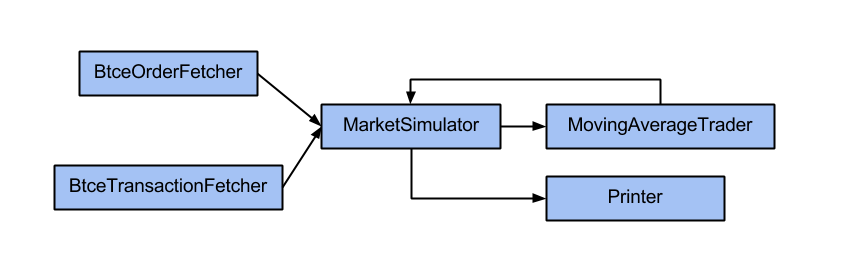
\includegraphics[width=\textwidth]{img/examples/btce}

The BTC-E fetchers get orders and transactions from \url{btc-e.com}, feed them to the market simulator. The market simulator generates transactions based on the bid and ask orders from the trader. The trader sends bid or ask orders to the market simulator based on the transactions received from the market simulator. The printer prints information about the market in the console.

\subsection{Forex Trading}

In this example, we demonstrate how to use the framework to experiment Forex trading with the \emph{MovingAverageTrader} on live Forex data. The component graph of this application is as follows:

\noindent
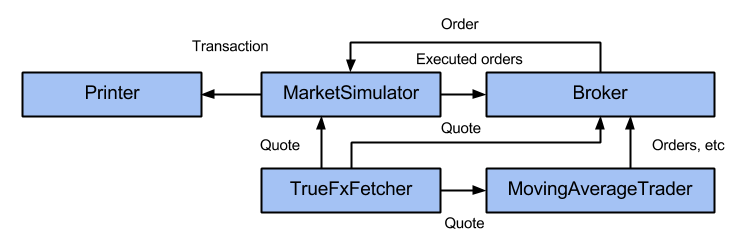
\includegraphics[width=\textwidth]{img/examples/forex-live}

In the component graph above, the fetcher gets live quotes data from \url{webrates.truefx.com}, and feeds them into the market simulator, trader and broker.

The trader makes sell and buy decisions based on the quotes received from the fetcher, and send them to the broker.

The broker receives orders from the trader, and forward them into the market simulator on behalf of the trader. Note that the usage of broker is optional, it's used here only for illustrating purpose.

The market simulator generates transactions based on the orders received from brokers, and sends the transaction result back to the broker.

\subsection{Replay}

In this example, we demonstrate how to use the framework to experiment Forex trading with the \emph{MovingAverageTrader} on history Forex data.

\noindent
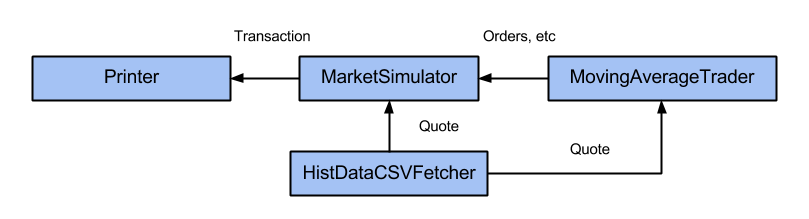
\includegraphics[width=\textwidth]{img/examples/forex-replay}

In the component graph above, the \emph{HistDataCSVFetcher} reads history quotes from CSV files, and send them to the market simulator and trader.

The trader produces ask or bid orders based on the quotes data, and sends them to the market simulator. The market simulator generates transactions based on the orders received from the trader.

The market simulator generates transactions based on received orders, and sends the transactions to the printer, which in turn prints them in the console.

%% \subsection{Simulation with Multiple Traders}

%% Multiple trader simulation in a virtual market.

\section{Simulation}
Besides the opportunity to tune strategies on historical and live data we aim to
create our own market simulation, meaning that prices are no longer defined 
externally but evolve as a result of interplays between the entities we implemented.
The purpose of this feature is to provide users with the opportunity to construct
complete and running ecosystems.

\subsection{Simplifying the Real Market}
Our project implements essential parts of the foreign exchange market.
In order to set up a basic market simulator we make the following
simplifications:

\begin{itemize}
    \item traders can only trade one symbol
    \item instruments are restricted to spot transactions
        \footnote{Referring to \url{http://www.newyorkfed.org/fxc/volumesurvey/explanatory_notes.html},
        instruments
        are product types available on the forex market, namely spot transactions, outright
        forwards, foreign exchange swaps and currency options. \textit{Spot transactions are single 
        outright transactions that involve the exchange of two currencies at a rate agreed 
        to on the date of the contract for value or delivery within two business days, including 
        U.S. dollar-Canadian dollar (USD-CAD) transactions delivered within one day).}

        All the other instruments involve contracts over a longer period of time and are
        currently not available.}


    \item two counterparties are involved: nonfinancial customers and market makers
        \footnote{\url{http://www.forextraders.com/market-maker-forex-brokers.html}}
        (representing all financial customers)
    \item one market maker per symbol
\end{itemize}

\subsection{Initial Parameters}
Finding appropriate parameters to configure a simulation that reflects the
true market has become a difficult task since existing statistics focus on 
the effects of the market meaning the daily turnover or distribution of market
shares by symbol, trading center or large financial customers. These statistics
are to be seen as results of trading activities. However, this does not allow
us to infer the cause of trading activity. In order to configure a market
simulation in a way that it would reflect the evolution of a real market we 
need to find the cause of activities and therefore we have to answer key questions
such as ``how many people are involved?'' or ``what are their funds?''.

Since we are not able to answer these questions reliably and also since we cannot
instantiate an infinite number of traders we introduce a different concept to
initialize a simulation.

We assign money to traders and market makers in a certain currency (e.g. USD) and 
they receive the equivalent amount in the currency they need to trade their respective
symbol as sketched in Algorithm~\ref{alg:initfunds}.

\begin{algorithm}
\caption{Distribution of initial funds.}
\label{alg:initfunds}
\begin{algorithmic}[1]
    \Statex Given: distribution of annual income for a specific country
    \footnote{example distribution: \url{http://www.bfs.admin.ch/bfs/portal/en/index/themen/03/04/blank/key/lohnstruktur/lohnverteilung.html}}
    \Statex
    \ForAll{$s \in symbols$}
        \State  $n \gets$ defined number of nonfinancial $traders$
        \ForAll{$t \in traders(s)$}
            \State $income \gets$ sample of income distribution
            \State $funds(t) \gets income$
        \EndFor
        \State $funds(marketmaker(s)) \gets c \cdot \sum_{i=1}^n funds(traders(i))$
    \EndFor
\end{algorithmic}
\end{algorithm}

%1. define number of non-financial traders
%
%2. for each trader: assign initial funds as 1-year income according to a local income distribution (e.g. Switzerland: http://www.bfs.admin.ch/bfs/portal/en/index/themen/03/04/blank/key/lohnstruktur/lohnverteilung.html)
%
%3. compute market makers initial funds as sum(funds(all traders)) * scale
%

\subsection{Price Definition during Simulation}

When our system is running in pure simulation mode, meaning that ask and bid price is
not defined by historical or live data anymore, prices must also be determined by the
simulation. 

\subsubsection{Balanced Demand and Offer}
In general, ask and bid price are determined by limit orders. In the case where there
exist limit orders on both sides (ask and bid) the current ask price is defined by the
lowest sell offer and the current bid price is defined by the highest buy offer.

\subsubsection{Extreme Situations}
It might occur that there are no limit orders and traders still want to trade at the 
current market price. In order to provide a price definition in such extreme scenarios
a market maker is introduced. Consider the following scenarios.

%I might also have found a solution to "how is the price defined when there is nobody on the other side (offering when I want to buy or asking when I want to sell)?".
%here http://www.forextraders.com/market-maker-forex-brokers.html I read that each market maker defines its own spread, which I understand the following way:
%
If there are only sellers and no buyers:
\begin{itemize}
    \item the \textit{ask} price is well defined as the lowest ask offer but the bid price is not
    \item the market maker defines the \textit{bid} price by applying its own spread to the lowest ask price
    \item selling at market price means selling to the market maker for the lowest \textit{ask price MINUS the spread}
\end{itemize}

If there are only buyers and no sellers:
\begin{itemize}
    \item the \textit{bid} price is well defined as the highest bid offer but the ask price is not
    \item the market maker defines the \textit{ask} price by applying its own spread to the highest bid price
    \item buying at market price means buying from the market maker at the highest \textit{bid price PLUS the spread}
\end{itemize}

If there are no limit orders at all:
\begin{itemize}
    \item ask and bid price stay constant
    \item random traders hopefully prevent the simulation from freezing
    \item optional: market maker could reduce spread, i.e. offer a higher bid price
    or a lower ask price
\end{itemize}

In any case where the prices are defined, but there is not enough capacity to buy the
volume some trader wishes to sell (or there is not enough offer to fulfill the demands
of a buying trader), the market maker buys (or sells) the remaining volume. Thereby the
assumption of permanent liquidity at the current market price is given as long as the
market maker has enough funds (which can be controlled through the scale parameter $c$
at init time.

The above covers the extreme scenarios. Still, one particular problem might arise that
does not occur in reality: given the buyers-only scenario, a single trader changing
their mind could make the market maker collapse. By introducing the only ask order (for a low volume) at 
a ridiculously low price it would define the ask price naturally and thereby force
the market maker to sell at this low price and eventually lose all its belongings
while selling at bad prices.

A similarly ill-posed problem occurs in a sellers-only market when a single trader
decides to make an extremely high bid order (for a low volume) that forces the market
maker to provide the respective bid price and eventually spend all its funds at buying
overpriced offers.

\subsection{Outline}
The software developed in this project is designed in a modular way. Hence, it is open
to adding new strategies and components. Extending the latter is particularly 
promising since the complexity of a real market is by far not fully covered yet. The next
important components are central banks. Since they fix interest rates on currencies 
they function as important indicators for strategies. Continuously implementing more
real actors will make the simulation more realistic and bring it closer to the goal 
of reflecting the actual market.


%
%\subsection{Brain Storm}
%
%Market Simulation Research
%
%[1] http://www.tpc.org/tpc_documents_current_versions/pdf/tpce-v1.14.0.pdf
%[2] www.swissquote.com
%[3] http://vantagepointtrading.com/daily-forex-stats
%[4] http://www.bis.org/publ/qtrpdf/r_qt1312e.pdf
%[5] turnovers by counterparty and currency pairs:
%http://www.reuters.com/article/2013/09/05/bis-survey-volumes-idUSL6N0GZ34R20130905
%
%[6] largest forex centers:
%http://countingpips.com/fx/2011/08/8-largest-forex-trading-centers-in-the-world/
%
%[7] directional trading volume:
%http://www.dailyfx.com/forex/technical/article/special_report/2015/04/13/forex-introducing-volume-by-price.html
%
%[8] https://mahifx.com/blog/50-fascinating-facts-about-forex
%
%[9] largest brokers by volume:
%http://www.myfxbook.com/forex-broker-volume
%
%[10] volume survey (North America) with explanation
%http://www.newyorkfed.org/fxc/volumesurvey/explanatory_notes.html
%
%[11] forex glossary
%http://www.cmsfx.com/en/forex-education/Forex-Glossary/ask-price/
%
%[12] salary distribution switzerland
%http://www.bfs.admin.ch/bfs/portal/en/index/themen/03/04/blank/key/lohnstruktur/lohnverteilung.html
%
%[13] explanation of market makers
%http://www.forextraders.com/market-maker-forex-brokers.html
%
%p.47 
%- Entity Relationships
%- Trade Types
%- run historical data for 300 business days before simulation starts
%
%Wanted:
%- trader initial funds -> half of annual income according to [12]?
%- broker initial funds (for leverage trades)
%- market maker funds
%- number of traders per currency pair
%- one market maker per currency pair?


%!TEX root = ../guide.tex

\section{Distributed setup}

One main characteristic of the Akka actor model is that each actor is solely responsible for maintaining its state, which is completely insulated from the external world. This way, we protect ourselves from synchronization problems and are allowed to run highly parallelized code.\\
Moreover, Akka has built-in \textit{remoting}\footnote{\url{http://doc.akka.io/docs/akka/snapshot/scala/remoting.html}} capabilities: actors can be instantiated remotely while maintaining referential transparency. Therefore, with minimal modifications to our initial codebase, we were able to run a distributed deployment of our system.\\

We demonstrate this feature using eight virtual machines (VM) from the \textit{Microsoft Azure}\footnote{\url{https://azure.microsoft.com/}} cloud. Each VM has very little requirements, as it needs only be accessible from the exterior world through the network and be able to run the Java Runtime Environment. The short script \texttt{vm-prepare.sh} contains all that is needed to make a mint Ubuntu system ready to run our code.

Finally, \texttt{workerctl.sh} provides useful commands for worker control, such as start / stop / restart. Executing \texttt{workerctl.sh start} will start a host actor system which will wait to receive commands from a master system. The latter can be started simply from your own machine, e.g. by running \texttt{ch.epfl.ts.optimization.RemotingMasterRunner}. Components are created and watched from the master onto the workers, which is responsible in this case for tracking the performance of each Trader instance and picking the best one at the end of the run.


\end{document}
